
%% bare_conf.tex
%% V1.3
%% 2007/01/11
%% by Michael Shell
%% See:
%% http://www.michaelshell.org/
%% for current contact information.
%%
%% This is a skeleton file demonstrating the use of IEEEtran.cls
%% (requires IEEEtran.cls version 1.7 or later) with an IEEE conference paper.
%%
%% Support sites:
%% http://www.michaelshell.org/tex/ieeetran/
%% http://www.ctan.org/tex-archive/macros/latex/contrib/IEEEtran/
%% and
%% http://www.ieee.org/

%%*************************************************************************
%% Legal Notice:
%% This code is offered as-is without any warranty either expressed or
%% implied; without even the implied warranty of MERCHANTABILITY or
%% FITNESS FOR A PARTICULAR PURPOSE!
%% User assumes all risk.
%% In no event shall IEEE or any contributor to this code be liable for
%% any damages or losses, including, but not limited to, incidental,
%% consequential, or any other damages, resulting from the use or misuse
%% of any information contained here.
%%
%% All comments are the opinions of their respective authors and are not
%% necessarily endorsed by the IEEE.
%%
%% This work is distributed under the LaTeX Project Public License (LPPL)
%% ( http://www.latex-project.org/ ) version 1.3, and may be freely used,
%% distributed and modified. A copy of the LPPL, version 1.3, is included
%% in the base LaTeX documentation of all distributions of LaTeX released
%% 2003/12/01 or later.
%% Retain all contribution notices and credits.
%% ** Modified files should be clearly indicated as such, including  **
%% ** renaming them and changing author support contact information. **
%%
%% File list of work: IEEEtran.cls, IEEEtran_HOWTO.pdf, bare_adv.tex,
%%                    bare_conf.tex, bare_jrnl.tex, bare_jrnl_compsoc.tex
%%*************************************************************************

% *** Authors should verify (and, if needed, correct) their LaTeX system  ***
% *** with the testflow diagnostic prior to trusting their LaTeX platform ***
% *** with production work. IEEE's font choices can trigger bugs that do  ***
% *** not appear when using other class files.                            ***
% The testflow support page is at:
% http://www.michaelshell.org/tex/testflow/



% Note that the a4paper option is mainly intended so that authors in
% countries using A4 can easily print to A4 and see how their papers will
% look in print - the typesetting of the document will not typically be
% affected with changes in paper size (but the bottom and side margins will).
% Use the testflow package mentioned above to verify correct handling of
% both paper sizes by the user's LaTeX system.
%
% Also note that the "draftcls" or "draftclsnofoot", not "draft", option
% should be used if it is desired that the figures are to be displayed in
% draft mode.
%
\documentclass[10pt, conference, compsocconf]{IEEEtran}
% Add the compsocconf option for Computer Society conferences.
%
% If IEEEtran.cls has not been installed into the LaTeX system files,
% manually specify the path to it like:
% \documentclass[conference]{../sty/IEEEtran}

%\usepackage[numbers, sort, compress]{natbib}
\usepackage{graphicx}
\usepackage{amsmath}
\usepackage{amssymb}
\usepackage{color}
\usepackage{ifpdf}
%\usepackage{mdwlist}

%\usepackage{dcolumn}
\usepackage{float}
\usepackage[utf8]{inputenc}
\usepackage{multirow}
\usepackage{rotating}
\usepackage{subfigure}

\usepackage{moresize}
%\usepackage{setspace}

%\usepackage[numbers, sort, compress]{natbib}
%\usepackage{latex8}
%\usepackage{float}
%\usepackage{times}    
\usepackage{url}
\usepackage{booktabs}
\usepackage{listings}   
\usepackage{paralist}    
\usepackage{wrapfig}    
%\usepackage[footnotesize,it]{caption}
\usepackage{multirow}
\usepackage{ifpdf}
%\usepackage{srcltx}
%\usepackage{subfigure}
\usepackage{xspace}
\usepackage{keyval}  
\usepackage{color}

\definecolor{listinggray}{gray}{0.95}
\definecolor{darkgray}{gray}{0.7}
\definecolor{commentgreen}{rgb}{0, 0.4, 0}
\definecolor{darkblue}{rgb}{0, 0, 0.4}
\definecolor{middleblue}{rgb}{0, 0, 0.7}
\definecolor{darkred}{rgb}{0.4, 0, 0}
\definecolor{brown}{rgb}{0.5, 0.5, 0}
\definecolor{dkgreen}{rgb}{0,0.5,0}
\definecolor{orange}{rgb}{1,.5,0}
\definecolor{dandelion}{cmyk}{0,0.29,0.84,0}

\usepackage[normalem]{ulem}
\makeatletter
\def\cyanuwave{\bgroup \markoverwith{\lower3.5\p@\hbox{\sixly \textcolor{cyan}{\char58}}}\ULon}
\def\reduwave{\bgroup \markoverwith{\lower3.5\p@\hbox{\sixly \textcolor{red}{\char58}}}\ULon}
\def\blueuwave{\bgroup \markoverwith{\lower3.5\p@\hbox{\sixly \textcolor{blue}{\char58}}}\ULon}
\font\sixly=lasy6 % does not re-load if already loaded, so no memory problem.
\makeatother


%\usepackage{xcolor}
\newif\ifdraft
\drafttrue
\ifdraft
 \newcommand{\N}[1]{\textbf{NOTE: #1}\xspace}
 \newcommand{\jhanote}[1]{ {\textcolor{red} { ***SJ: #1 }}}
 \newcommand{\katznote}[1]{ {\textcolor{blue} { ***DSK: #1 }}}
 \newcommand{\mtnote}[1]{ {\textcolor{orange} { ***MT: #1 }}}
 \newcommand{\jonnote}[1]{ {\textcolor{dkgreen} { ***JW: #1 }}}
  \newcommand{\aanote}[1]{ {\textcolor{dkgreen} { ***AA: #1 }}}
 \newcommand{\note}[1]{ {\textcolor{brown} { *** #1 }}}
\else
 \newcommand{\N}[1]{}
 \newcommand{\jhanote}[1]{}
 \newcommand{\katznote}[1]{}
 \newcommand{\mtnote}[1]{}
 \newcommand{\jonnote}[1]{}
 \newcommand{\note}[1]{}
\fi

\newif\ifdraft
%\drafttrue
\ifdraft
\newcommand{\terminology}[1]{ {\textcolor{red} {(Terminology used: \textbf{#1}) }}}
\newcommand{\owave}[1]{ {\cyanuwave{#1}}}
\newcommand{\jwave}[1]{ {\reduwave{#1}}}
\newcommand{\alwave}[1]{ {\blueuwave{#1}}}
\newcommand{\alnote}[1]{ {\textcolor{blue} { ***andreL: #1 }}}
\newcommand{\amnote}[1]{ {\textcolor{blue} { ***andreM: #1 }}}
\newcommand{\smnote}[1]{ {\textcolor{brown} { ***sharath: #1 }}}
\newcommand{\pmnote}[1]{ {\textcolor{brown} { ***Pradeep: #1 }}}
\newcommand{\msnote}[1]{ {\textcolor{cyan} { ***mark: #1 }}}
\newcommand{\mrnote}[1]{ {\textcolor{purple} { ***melissa: #1 }}}
%\newcommand{\mtnote}[1]{ {\textcolor{orange} { ***matteo: #1 }}}
\else
\newcommand{\onote}[1]{}
\newcommand{\terminology}[1]{}
\newcommand{\owave}[1]{#1}
\newcommand{\jwave}[1]{#1}
\newcommand{\alnote}[1]{}
\newcommand{\amnote}[1]{}
\newcommand{\athotanote}[1]{}
\newcommand{\smnote}[1]{}
\newcommand{\pmnote}[1]{}
\newcommand{\msnote}[1]{}
\newcommand{\mrnote}[1]{}
\newcommand{\aznote}[1]{}
%\newcommand{\mtnote}[1]{}
\fi

\newcommand{\cloud}{cloud\xspace}
\newcommand{\clouds}{clouds\xspace}
\newcommand{\pilot}{Pilot\xspace}
\newcommand{\pilots}{Pilots\xspace}
\newcommand{\pilotjob}{Pilot-Job\xspace}
\newcommand{\pilotjobs}{Pilot-Jobs\xspace}
\newcommand{\pilotcompute}{Pilot-Compute\xspace}
\newcommand{\pilotcomputedescription}{Pilot-Compute Description\xspace}
\newcommand{\pilotdescription}{Pilot-Description\xspace}
\newcommand{\pilotcomputes}{Pilot-Computes\xspace}
\newcommand{\pilotdata}{Pilot-Data\xspace}
\newcommand{\pilotdatadescription}{Pilot-Data Description\xspace}
\newcommand{\pilotdataservice}{Pilot-Data Service\xspace}
\newcommand{\pilotcomputeservice}{Pilot-Compute Service\xspace}
\newcommand{\computedataservice}{Compute-Data Service\xspace}
\newcommand{\computeunitdescription}{Compute-Unit Description\xspace}
\newcommand{\dataunitdescription}{Data-Unit Description\xspace}
\newcommand{\pilotmapreduce}{PilotMapReduce\xspace}
\newcommand{\mrmg}{MR-Manager\xspace}
\newcommand{\pstar}{P*\xspace}
\newcommand{\pd}{PD\xspace}
\newcommand{\pc}{PC\xspace}
\newcommand{\pcs}{PCs\xspace}
\newcommand{\pj}{PJ\xspace}
\newcommand{\pjs}{PJs\xspace}
\newcommand{\pds}{Pilot Data Service\xspace}
\newcommand{\computeunit}{Compute-Unit\xspace}
\newcommand{\computeunits}{Compute-Units\xspace}
\newcommand{\dataunit}{Data-Unit\xspace}
\newcommand{\dataunits}{Data-Units\xspace}
\newcommand{\du}{DU\xspace}
\newcommand{\dus}{DUs\xspace}
\newcommand{\dud}{DUD\xspace}
\newcommand{\cu}{CU\xspace}
\newcommand{\cus}{CUs\xspace}
\newcommand{\cud}{CUD\xspace}
\newcommand{\su}{SU\xspace}
\newcommand{\sus}{SUs\xspace}
\newcommand{\schedulableunit}{Schedulable Unit\xspace}
\newcommand{\schedulableunits}{Schedulable Units\xspace}
\newcommand{\cc}{c\&c\xspace}
\newcommand{\CC}{C\&C\xspace}
\newcommand{\up}{\vspace*{-1em}}
\newcommand{\upp}{\vspace*{-0.5em}}
\newcommand{\numrep}{8 }
\newcommand{\samplenum}{4 }
\newcommand{\tmax}{$T_{max}$ }
\newcommand{\tc}{$T_{C}$ }
\newcommand{\tcnsp}{$T_{C}$}
\newcommand{\bj}{BigJob\xspace}
\newcommand{\irods}{iRODS\xspace}

\newcommand{\I}[1]{\textit{#1}\xspace}
\newcommand{\B}[1]{\textbf{#1}\xspace}
\newcommand{\T}[1]{\texttt{#1}\xspace}
\newcommand{\C}[1]{\textsc{#1}\xspace}

\newcommand{\mr}[1]{\multirow{2}{*}{#1}}%
\newcommand{\mc}[2]{\multicolumn{#1}{l}{#2}}

\lstdefinestyle{myListing}{
  frame=single,   
  backgroundcolor=\color{listinggray},  
  %float=t,
  language=C,       
  basicstyle=\ttfamily \footnotesize,
  breakautoindent=true,
  breaklines=true
  tabsize=2,
  captionpos=b,  
  aboveskip=0em,
  belowskip=-2em,
  %numbers=left, 
  %numberstyle=\tiny
}      

\lstdefinestyle{myPythonListing}{
  frame=single,   
  backgroundcolor=\color{listinggray},  
  %float=t,
  language=Python,       
  basicstyle=\ttfamily \scriptsize,
  breakautoindent=true,
  breaklines=true
  tabsize=2,
  captionpos=b,  
  %numbers=left, 
  %numberstyle=\tiny
}



%  \setlength{\parskip}{0.05ex} % 1ex plus 0.5ex minus 0.2ex}
%  \setlength{\parsep}{0pt}
%  %\setlength{\headsep}{0pt}
%  \setlength{\topskip}{0pt}
%  \setlength{\topmargin}{0pt}
%  %\setlength{\topsep}{0pt}
%  \setlength{\partopsep}{0pt}

% This is now the recommended way for checking for PDFLaTeX:


\ifpdf
\DeclareGraphicsExtensions{.pdf, .jpg, .tif}
\else
\DeclareGraphicsExtensions{.ps,  .eps, .jpg}
\fi

\tolerance=1000
\hyphenpenalty=10


% Some very useful LaTeX packages include:
% (uncomment the ones you want to load)


% *** MISC UTILITY PACKAGES ***
%
%\usepackage{ifpdf}
% Heiko Oberdiek's ifpdf.sty is very useful if you need conditional
% compilation based on whether the output is pdf or dvi.
% usage:
% \ifpdf
%   % pdf code
% \else
%   % dvi code
% \fi
% The latest version of ifpdf.sty can be obtained from:
% http://www.ctan.org/tex-archive/macros/latex/contrib/oberdiek/
% Also, note that IEEEtran.cls V1.7 and later provides a builtin
% \ifCLASSINFOpdf conditional that works the same way.
% When switching from latex to pdflatex and vice-versa, the compiler may
% have to be run twice to clear warning/error messages.






% *** CITATION PACKAGES ***
%
%\usepackage{cite}
% cite.sty was written by Donald Arseneau
% V1.6 and later of IEEEtran pre-defines the format of the cite.sty package
% \cite{} output to follow that of IEEE. Loading the cite package will
% result in citation numbers being automatically sorted and properly
% "compressed/ranged". e.g., [1], [9], [2], [7], [5], [6] without using
% cite.sty will become [1], [2], [5]--[7], [9] using cite.sty. cite.sty's
% \cite will automatically add leading space, if needed. Use cite.sty's
% noadjust option (cite.sty V3.8 and later) if you want to turn this off.
% cite.sty is already installed on most LaTeX systems. Be sure and use
% version 4.0 (2003-05-27) and later if using hyperref.sty. cite.sty does
% not currently provide for hyperlinked citations.
% The latest version can be obtained at:
% http://www.ctan.org/tex-archive/macros/latex/contrib/cite/
% The documentation is contained in the cite.sty file itself.






% *** GRAPHICS RELATED PACKAGES ***
%
\ifCLASSINFOpdf
  % \usepackage[pdftex]{graphicx}
  % declare the path(s) where your graphic files are
  % \graphicspath{{../pdf/}{../jpeg/}}
  % and their extensions so you won't have to specify these with
  % every instance of \includegraphics
  % \DeclareGraphicsExtensions{.pdf,.jpeg,.png}
\else
  % or other class option (dvipsone, dvipdf, if not using dvips). graphicx
  % will default to the driver specified in the system graphics.cfg if no
  % driver is specified.
  % \usepackage[dvips]{graphicx}
  % declare the path(s) where your graphic files are
  % \graphicspath{{../eps/}}
  % and their extensions so you won't have to specify these with
  % every instance of \includegraphics
  % \DeclareGraphicsExtensions{.eps}
\fi
% graphicx was written by David Carlisle and Sebastian Rahtz. It is
% required if you want graphics, photos, etc. graphicx.sty is already
% installed on most LaTeX systems. The latest version and documentation can
% be obtained at:
% http://www.ctan.org/tex-archive/macros/latex/required/graphics/
% Another good source of documentation is "Using Imported Graphics in
% LaTeX2e" by Keith Reckdahl which can be found as epslatex.ps or
% epslatex.pdf at: http://www.ctan.org/tex-archive/info/
%
% latex, and pdflatex in dvi mode, support graphics in encapsulated
% postscript (.eps) format. pdflatex in pdf mode supports graphics
% in .pdf, .jpeg, .png and .mps (metapost) formats. Users should ensure
% that all non-photo figures use a vector format (.eps, .pdf, .mps) and
% not a bitmapped formats (.jpeg, .png). IEEE frowns on bitmapped formats
% which can result in "jaggedy"/blurry rendering of lines and letters as
% well as large increases in file sizes.
%
% You can find documentation about the pdfTeX application at:
% http://www.tug.org/applications/pdftex





% *** MATH PACKAGES ***
%
%\usepackage[cmex10]{amsmath}
% A popular package from the American Mathematical Society that provides
% many useful and powerful commands for dealing with mathematics. If using
% it, be sure to load this package with the cmex10 option to ensure that
% only type 1 fonts will utilized at all point sizes. Without this option,
% it is possible that some math symbols, particularly those within
% footnotes, will be rendered in bitmap form which will result in a
% document that can not be IEEE Xplore compliant!
%
% Also, note that the amsmath package sets \interdisplaylinepenalty to 10000
% thus preventing page breaks from occurring within multiline equations. Use:
%\interdisplaylinepenalty=2500
% after loading amsmath to restore such page breaks as IEEEtran.cls normally
% does. amsmath.sty is already installed on most LaTeX systems. The latest
% version and documentation can be obtained at:
% http://www.ctan.org/tex-archive/macros/latex/required/amslatex/math/





% *** SPECIALIZED LIST PACKAGES ***
%
%\usepackage{algorithmic}
% algorithmic.sty was written by Peter Williams and Rogerio Brito.
% This package provides an algorithmic environment fo describing algorithms.
% You can use the algorithmic environment in-text or within a figure
% environment to provide for a floating algorithm. Do NOT use the algorithm
% floating environment provided by algorithm.sty (by the same authors) or
% algorithm2e.sty (by Christophe Fiorio) as IEEE does not use dedicated
% algorithm float types and packages that provide these will not provide
% correct IEEE style captions. The latest version and documentation of
% algorithmic.sty can be obtained at:
% http://www.ctan.org/tex-archive/macros/latex/contrib/algorithms/
% There is also a support site at:
% http://algorithms.berlios.de/index.html
% Also of interest may be the (relatively newer and more customizable)
% algorithmicx.sty package by Szasz Janos:
% http://www.ctan.org/tex-archive/macros/latex/contrib/algorithmicx/




% *** ALIGNMENT PACKAGES ***
%
%\usepackage{array}
% Frank Mittelbach's and David Carlisle's array.sty patches and improves
% the standard LaTeX2e array and tabular environments to provide better
% appearance and additional user controls. As the default LaTeX2e table
% generation code is lacking to the point of almost being broken with
% respect to the quality of the end results, all users are strongly
% advised to use an enhanced (at the very least that provided by array.sty)
% set of table tools. array.sty is already installed on most systems. The
% latest version and documentation can be obtained at:
% http://www.ctan.org/tex-archive/macros/latex/required/tools/


%\usepackage{mdwmath}
%\usepackage{mdwtab}
% Also highly recommended is Mark Wooding's extremely powerful MDW tools,
% especially mdwmath.sty and mdwtab.sty which are used to format equations
% and tables, respectively. The MDWtools set is already installed on most
% LaTeX systems. The lastest version and documentation is available at:
% http://www.ctan.org/tex-archive/macros/latex/contrib/mdwtools/


% IEEEtran contains the IEEEeqnarray family of commands that can be used to
% generate multiline equations as well as matrices, tables, etc., of high
% quality.


%\usepackage{eqparbox}
% Also of notable interest is Scott Pakin's eqparbox package for creating
% (automatically sized) equal width boxes - aka "natural width parboxes".
% Available at:
% http://www.ctan.org/tex-archive/macros/latex/contrib/eqparbox/





% *** SUBFIGURE PACKAGES ***
%\usepackage[tight,footnotesize]{subfigure}
% subfigure.sty was written by Steven Douglas Cochran. This package makes it
% easy to put subfigures in your figures. e.g., "Figure 1a and 1b". For IEEE
% work, it is a good idea to load it with the tight package option to reduce
% the amount of white space around the subfigures. subfigure.sty is already
% installed on most LaTeX systems. The latest version and documentation can
% be obtained at:
% http://www.ctan.org/tex-archive/obsolete/macros/latex/contrib/subfigure/
% subfigure.sty has been superceeded by subfig.sty.



%\usepackage[caption=false]{caption}
%\usepackage[font=footnotesize]{subfig}
% subfig.sty, also written by Steven Douglas Cochran, is the modern
% replacement for subfigure.sty. However, subfig.sty requires and
% automatically loads Axel Sommerfeldt's caption.sty which will override
% IEEEtran.cls handling of captions and this will result in nonIEEE style
% figure/table captions. To prevent this problem, be sure and preload
% caption.sty with its "caption=false" package option. This is will preserve
% IEEEtran.cls handing of captions. Version 1.3 (2005/06/28) and later
% (recommended due to many improvements over 1.2) of subfig.sty supports
% the caption=false option directly:
%\usepackage[caption=false,font=footnotesize]{subfig}
%
% The latest version and documentation can be obtained at:
% http://www.ctan.org/tex-archive/macros/latex/contrib/subfig/
% The latest version and documentation of caption.sty can be obtained at:
% http://www.ctan.org/tex-archive/macros/latex/contrib/caption/




% *** FLOAT PACKAGES ***
%
%\usepackage{fixltx2e}
% fixltx2e, the successor to the earlier fix2col.sty, was written by
% Frank Mittelbach and David Carlisle. This package corrects a few problems
% in the LaTeX2e kernel, the most notable of which is that in current
% LaTeX2e releases, the ordering of single and double column floats is not
% guaranteed to be preserved. Thus, an unpatched LaTeX2e can allow a
% single column figure to be placed prior to an earlier double column
% figure. The latest version and documentation can be found at:
% http://www.ctan.org/tex-archive/macros/latex/base/



%\usepackage{stfloats}
% stfloats.sty was written by Sigitas Tolusis. This package gives LaTeX2e
% the ability to do double column floats at the bottom of the page as well
% as the top. (e.g., "\begin{figure*}[!b]" is not normally possible in
% LaTeX2e). It also provides a command:
%\fnbelowfloat
% to enable the placement of footnotes below bottom floats (the standard
% LaTeX2e kernel puts them above bottom floats). This is an invasive package
% which rewrites many portions of the LaTeX2e float routines. It may not work
% with other packages that modify the LaTeX2e float routines. The latest
% version and documentation can be obtained at:
% http://www.ctan.org/tex-archive/macros/latex/contrib/sttools/
% Documentation is contained in the stfloats.sty comments as well as in the
% presfull.pdf file. Do not use the stfloats baselinefloat ability as IEEE
% does not allow \baselineskip to stretch. Authors submitting work to the
% IEEE should note that IEEE rarely uses double column equations and
% that authors should try to avoid such use. Do not be tempted to use the
% cuted.sty or midfloat.sty packages (also by Sigitas Tolusis) as IEEE does
% not format its papers in such ways.





% *** PDF, URL AND HYPERLINK PACKAGES ***
%
%\usepackage{url}
% url.sty was written by Donald Arseneau. It provides better support for
% handling and breaking URLs. url.sty is already installed on most LaTeX
% systems. The latest version can be obtained at:
% http://www.ctan.org/tex-archive/macros/latex/contrib/misc/
% Read the url.sty source comments for usage information. Basically,
% \url{my_url_here}.





% *** Do not adjust lengths that control margins, column widths, etc. ***
% *** Do not use packages that alter fonts (such as pslatex).         ***
% There should be no need to do such things with IEEEtran.cls V1.6 and later.
% (Unless specifically asked to do so by the journal or conference you plan
% to submit to, of course. )


% correct bad hyphenation here
\hyphenation{op-tical net-works semi-conduc-tor}


\newcommand{\sarp}[1]{{\color{green}\textit{sarp: {#1}}}}


\begin{document}
%
% paper title
% can use linebreaks \\ within to get better formatting as desired
\title{Everthing you wanted to know about PanDA but were truly truly afraid to ask}


% author names and affiliations
% use a multiple column layout for up to two different
% affiliations

\author{\IEEEauthorblockN{Authors Name/s per 1st Affiliation (Author)}
\IEEEauthorblockA{line 1 (of Affiliation): dept. name of organization\\
line 2: name of organization, acronyms acceptable\\
line 3: City, Country\\
line 4: Email: name@xyz.com}
\and
\IEEEauthorblockN{Authors Name/s per 2nd Affiliation (Author)}
\IEEEauthorblockA{line 1 (of Affiliation): dept. name of organization\\
line 2: name of organization, acronyms acceptable\\
line 3: City, Country\\
line 4: Email: name@xyz.com}
}

% conference papers do not typically use \thanks and this command
% is locked out in conference mode. If really needed, such as for
% the acknowledgment of grants, issue a \IEEEoverridecommandlockouts
% after \documentclass

% for over three affiliations, or if they all won't fit within the width
% of the page, use this alternative format:
%
%\author{\IEEEauthorblockN{Michael Shell\IEEEauthorrefmark{1},
%Homer Simpson\IEEEauthorrefmark{2},
%James Kirk\IEEEauthorrefmark{3},
%Montgomery Scott\IEEEauthorrefmark{3} and
%Eldon Tyrell\IEEEauthorrefmark{4}}
%\IEEEauthorblockA{\IEEEauthorrefmark{1}School of Electrical and Computer Engineering\\
%Georgia Institute of Technology,
%Atlanta, Georgia 30332--0250\\ Email: see http://www.michaelshell.org/contact.html}
%\IEEEauthorblockA{\IEEEauthorrefmark{2}Twentieth Century Fox, Springfield, USA\\
%Email: homer@thesimpsons.com}
%\IEEEauthorblockA{\IEEEauthorrefmark{3}Starfleet Academy, San Francisco, California 96678-2391\\
%Telephone: (800) 555--1212, Fax: (888) 555--1212}
%\IEEEauthorblockA{\IEEEauthorrefmark{4}Tyrell Inc., 123 Replicant Street, Los Angeles, California 90210--4321}}

% use for special paper notices
%\IEEEspecialpapernotice{(Invited Paper)}

% make the title area
\maketitle


\begin{abstract}
 Experiments at the Large Hadron Collider (LHC) face unprecedented   computing   challenges.  Heterogeneous  resources are distributed worldwide, thousands of physicists analyzing the data need remote access to hundreds of computing  sites, the volume of processed data is beyond  the exabyte  scale, and data processing requires more than billions of hours of computing usage per year. The PanDA (Production and Distributed Analysis) system was developed to meet the scale and complexity of LHC distributed computing for the ATLAS experiment. In the process, the old batch job paradigm of computing in HEP was discarded in favor of a far more flexible and scalable model. The success of PanDA at the LHC is leading to widespread adoption and testing by other experiments.  PanDA is  the first exascale  workload management   system  in HEP,  already operating  at a million computing jobs per day, and processing over an exabyte of data in
2013. We will describe the design and implementation  of PanDA, present  data on the performance  of PanDA at the LHC,  and discuss plans  for future  evolution of the system  to meet new challenges of scale, heterogeneity  and increasing user base.
\end{abstract}

\begin{IEEEkeywords}
TBD.
\end{IEEEkeywords}


% For peer review papers, you can put extra information on the cover
% page as needed:
% \ifCLASSOPTIONpeerreview
% \begin{center} \bfseries EDICS Category: 3-BBND \end{center}
% \fi
%
% For peerreview papers, this IEEEtran command inserts a page break and
% creates the second title. It will be ignored for other modes.
\IEEEpeerreviewmaketitle

% ----------------------------------------------------------------------------
% I
% ----------------------------------------------------------------------------
\section{Introduction}\label{sec:intro}
The Large Hadron Collider (LHC) is created  to explore the fundamental  properties  of matter for the next decades. Since LHC start-up in 2009, the experiments has collected and distributed hundreds  of  petabytes  of  data worldwide to hundreds of computer centers. Thousands of physicists analyze petascale  data volumes daily. One of  the LHC experiments  the ATLAS  \cite{Aad:2008}  utilizes the PanDA  workload management system \cite{Maeno2011} (WMS) for distributed data processing and analysis. The ATLAS Computing model \cite{Atlas2005} is based on a Grid paradigm \cite{Foster:1998}, with multilevel, hierarchically distributed computing  and storage resources. Acronym  PanDa stands for Production  and Distributed Analysis, the system  has  been developed to meet growing ATLAS production and analysis requirements for a data-driven  workload  management system capable of operating at LHC data processing scale.
PanDA has a highly scalable architecture. Scalability  has been demonstrated in ATLAS through the rapid increase in usage over the past several years of operations, and is expected to meet the continuously growing number of jobs over the next decade. PanDA  was designed to have the flexibility to adapt to emerging computing  technologies in processing,  storage, networking  as well as the underlying software stack (middleware). This flexibility has also been successfully demonstrated through the past six years of evolving  technologies adapted by computing centers in ATLAS which span many continents and yet are seamlessly integrated into PanDA.
PanDA  manages a wide spectrum of workloads, ranging from raw data processing to Monte Carlo simulation and user analysis, while actively evolving to meet rapidly changing science needs.  Today, it  serves several  thousand users, successfully managing job distribution to hundreds of ATLAS sites with more than 100,000 CPU cores  which process  more than a million jobs per day, Figure 1 shows  a  summary   of daily completed jobs on ATLAS Grid for the past 12 month.
\begin{figure}
\begin{center}
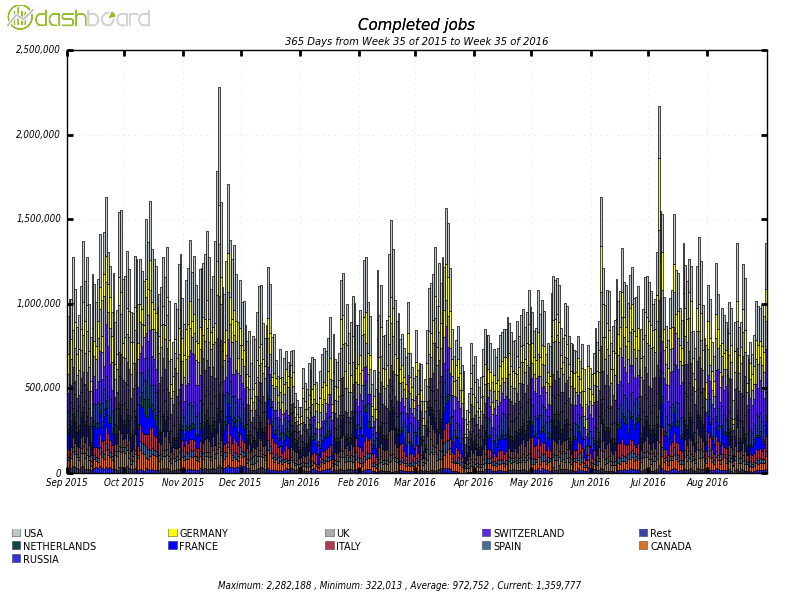
\includegraphics[width=\columnwidth]{figures/DailyJobs.png}
\caption{Daily completed jobs on ATLAS Grid\label{fig:daily}}
\end{center}
\end{figure}

--------------------------------------------------------------------
\begin{enumerate}
  \item Problem that has been solved: executing many applications on heterogeneous distributed resources.
  \item Why are WMS needed?
  \item Increasing importance of WMS w.r.t complex and scalable applications on heterogeneous distributed resources.
  \item \ldots
  \item Overview/Summary of paper.
\end{enumerate}

% ----------------------------------------------------------------------------
% II
% ----------------------------------------------------------------------------
\section{Background}
\label{sec:background}

\begin{enumerate}
  \item Brief overview of distributed CI.
  \item Workload vs Workflow. (DONE)
  \item Distinguish between WFMS and WLMS.
  \begin{enumerate}
    \item Role of Workload MS: help ``hide'' and federate heterogeneous resources.
  \end{enumerate}
\end{enumerate}

--------------------------------------------------------------------

\paragraph*{Workload Vs Workflow} The term ``workflow'' is used in many
disciplines with different meaning. In the field of scientific computing,
``workflow'' assumes different meanings depending on the characteristics of
the computation, of the software tools used to support this computation, and
of the resources on which it is performed. Further, a workflow may indicate a
whole application, a description of the computational process of that
application or, more commonly, a series of tasks related by data
dependences.

The lack of a consistent and shared definition of ``workflow'' hinders the
understanding of its properties and its relations with related concepts. For
example, we need to clarify the difference between ``workflow'', ``workload'',
``task'', or ``job'' but also between workflow template and instance, or
data-flow and control-flow. This clarification is precondition to specify
properly the design of software systems that support the execution of
scientific applications.

In this paper, we use the following definitions:

\begin{description}
  \item[Task.] A set of operations to be performed on a computing platform,
  alongside a description of the properties and dependences of those
  operations, and indications on how they should be executed and satisfied.
  \item[Workload.] A set of tasks that can be executed concurrently, possibly
  related by a set of relations. For example, tasks of a workload can share
  one or more input files or communicate during execution.
  \item[Workflow.] Set of workloads, related by a set of relations that define
  the order in which each workload can be executed. Data dependences are the
  most common relations among workloads, used to define the precedence among
  their executions. Note that, formally, a workload can have a single task.
\end{description}

Each task may have an arbitrary number of properties like number of cores,
executables, or input/output files. Tasks may have precedence relations
depending on their data dependences or any other type of dependency mandated
by the application algorithms. Tasks with precedence relations have to be
executed serially, otherwise tasks can be executed concurrently. A workload is
defined as a set of tasks that can be executed concurrently. As such, a
workflow can be composed by a set of workloads.

The terms ``task'' and ``job'' are also used inconsistently across communities
that perform scientific computing. In this paper, ``job'' refers to the entity
that is submitted to a local resource management system (LRMS), like a batch
system or a scheduler. As such, a task can become a job when is scheduled on a
resource that exposes a LRMS but can also become a virtual machine or a
container when bootstrapped on an infrastructure supporting virtualization.

Usually, workflows are represented as graphs where tasks are vertices and
their relations are edges~\cite{}. Often, graphs are supposed to be acyclic
but graphs with cycles have been used to represent workflows of
workflows~\cite{}. In this paper, a workflow template is a type of graph while
a workflow instance is a type of graph with a specific set of vertices and
edges. Further, a graph is ``abstract'' when no resource properties are
available for all vertices, ``concrete'' otherwise~\cite{}.

The distinction between an abstract and concrete graph highlights an important
element of the execution process of a workflow. Workflows can be specified
without indicating on what resources they should be executed. Accordingly, an
abstract graph can be interpreted as a formal description of the requirements
for the workflow execution. Once these requirements are matched by a set of
resource capabilities, the graph becomes concrete, i.e. a formal description
of the workflow execution process and its execution environment.

% ----------------------------------------------------------------------------
% III
% ----------------------------------------------------------------------------
\section{Related Work}
\label{sec:related}
\subsection{Alien}
Alien is a Workload and Data Management system composed of a 	set of middleware tools and services entirely based on web-services and standard protocols. Alien was originally developed for the ALICE experiment \cite{} but subsequently used by several virtual organizations \cite{}. 
%The system has been deployed in 2001 for distributed producti	on of Monte Carlo data, detector simulation and reconstruction.
Alien is composed of two type of services:
\begin{itemize}
\item
\emph{Central services}, these services are unique for each virtual organisation, therefore there is only one  configuration point for the management;
\item \emph{Site services}, they provide the interfacing to local resources and Grid services running on a VO-box;
\end{itemize}

The most important central services are:
\begin{itemize}
\item \emph{Job Manager}, a database that keeps track of all the jobs submitted to the system and their current execution status;
\item \emph{Brokers}, they are the core of task executions and data transfers; they receive tasks in form of JDL,  keep them ordered by priority and send them to the CE for execution;
\item \emph{Optimizers}, they are used to minimize the work of the Broker by scanning periodially the task queue and re-arranging the tasks in such a way that fairness and priority policies are guaranted;
\item \emph{Data Catalogue}, it keeps track of the scripts and files uploaded on Storage Elements.
\end{itemize}

%The Computing Agents are instead site services that monitor the local Computing Element, advertise site's capabilities and are responsible for submitting the JobAgents.

%Information about the status of the sites and central services, full job statistics and monitoring information are kept in a MonALISA repository.
%% CLUSTER MONITOR SHOULD BE EQUAL TO COMPUTING AGENT
%% Job Manager should be equal to TaskQueue
%% Process Monitor == PIlot????

The job execution in Alien is usually distributed over several sites. Each of these sites has at least one service called ClusterMonitor. On one side the Cluster Monitor is used to communicate with Central services (Job Manager and Broker), on the other side it can manage Computing Elements (CE) by starting and stopping them whenever it receives the signal.
The CE is the resource in charge of the execution of the jobs. A CE usually is associated with a batch queue and can send the jobs to the worker nodes controlled by the queue.

The CE asks the Broker for jobs to execute by sending its JDL. Once received the JDL, the Broker will try to match it with the JDL of the jobs in queue. If a match exists then the Broker sends the jobs JDL to the CE.
Immediately after receving a job JDL, the CE create a new service on the worker node called ProcessMonitor. This service allows the CE (and the rest of Alien services through the CE) to interact with the job while is running. 
This execution strategy is called ``pull mode'' due to the fact that CE asks for jobs.
It is worth to mention that more recent version of Alien implement exploit gLite and CE-CREAM. The latter allows the system to by-pass the broker during the job submission \cite{}. 

Alien uses the Job Description Language (JDL) to allow users to describe their workload task by task;  i.e.,  users can specify features such as task priorities, the level of parallelism (one core, multi-core, MPI etc..) and  also the DCR that should be targeted for the execution.

%Job submission is implemented by following the so-called ``pull mode'' which is composed of the following steps: 
%\begin{enumerate}
% \item the VO-Box monitors the status of the site queues through polls to the resource running on the CE; 
%\item  the Job Broker receives a report everytime slots become available; 
%\item  if the Task Queue is not empty, the Job Broker asks the VO-box to submit a number of Agents;
%\item finally, the JobAgents are submitted  to the site Computing Element either by way of that sends them back to the site Computing Element or, wherever available, directly through the CREAM interface on the CE itself.
%\end{enumerate}

\subsection{DIRAC} 
DIRAC (Distributed Infrastructure with Remote Agent Control) Workload and Data Management System is a software product, developed within the CERN LHCb project, to manage the processing of detector data, Monte Carlo simulations, and end-user analyses. 
DIRAC  architecture relies on four entities:
\begin{itemize}
\item \emph{Clients}: consist in a set of APIs that allows users to submit job requests. Clients interact directly with DIRAC central services.
\item \emph{Services}: serve Clients and Agents by performing crucial operations such as Job Management, Configuration, Bookkeping and Accounting.
\item \emph{Agents}: perform repetitive tasks like querying file catalogs,  monitoring of jobs on resources.
\item \emph{Resources}: they can be PC's, site cluters and Grids. Agents interact with them without distinction.
\end{itemize}
In the same way of Alien, DIRAC implements a pull scheduling. Furthermore DIRAC was the first WMS to exploit the concept of Pilot Agent on the Grid. 
Pilots Agents are gLite jobs that are submitted to the grid when jobs arrive into the WMS. 
DIRAC pilot system has four main logical components:
\begin{itemize}
\item a set of TaskQueues that collect tasks submitted by users, multiple TaskQueue being created depending on the requirements and ownership of the tasks;
\item a set of JobWrappers that are executed on the DCR to bind compute resources and execute tasks submitted by the users;
\item a set of TaskQueueDirectors that submits JobWrappers to target DCRs;
\item a MatchMaker that matches requests from JobWrappers to suitable tasks into TaskQeues.
\end{itemize}
The DIRAC execution model can be summarized in five
steps: 1. a user submits its workload in form of tasks to the WMS Job Manager; 2. submitted tasks are validated and added to a new or an existing TaskQueue, depending on the task properties; 3. TaskQueueDirector evaluates TaskQueues and a suitable number of JobWrappers are submitted to available
DCRs; 4. JobWrappers get instantiated on the DCRs and, then,  ask for tasks to the MatchMaker; 5. JobWrappers execute tasks while JobWrapper’s Watchdog monitor them.
TaskQueueDirectors deploy Pilots by getting a list of TaskQueues and calculating the number of pilot to submit  according to user priorities.
Once deployed on the compute resource, Pilots, a.k.a. JobWrappers, hold the resource in the form of single or multiple cores, spanning portions, whole, or multiple compute nodes. Pilots do not expose data capabilities although the system allows the user to perform both data staging and data replication. 
TaskQueues, TaskQueueDirectors, and the MatchMaker are implemented as services whereas the JobWrapper is implemented within the Agents together with the WatchDog. 

\subsection{HTCondor Glidein and GlideinWMS}
The HTCondor Glidein system  as part of
the HTCondor [153] software ecosystem. The HTCondor
Glidein is a pilot-based system to aggregate DCRs with
heterogeneous middleware into HTCondor resource pools.
The logical components of HTCondor relevant to the
Glidein system are: 
\begin{itemize}
\item \emph{Schedd}, a daemon that implement a queuing system that holds workload tasks;
\item \emph{Startd}, a  daemon to control the DCR resources. 
\item \emph{Collector}, holds references to all the active
Schedd/Startd daemons; 
\item \emph{Negotiator} matches tasks queued in a Schedd to resources handled by a Startd.
\end{itemize}
In
HTCondor Glidein has been complemented by Glidein-WMS, a Glidein-based workload management system thatautomates deployment and management of Glideins on multiple types of DCR middleware. GlideinWMS builds upon the
HTCondor Glidein system by adding the following logical components: 
\begin{itemize}
\item \emph{Glidein Factories} that submit tasks to the DCRs middleware;
\item a set of \emph{Virtual Organizations (VO) Frontend} daemons that match the tasks on one or more Schedd to the resource attributes;
\item a \emph{Collector} that holds references to all the active Glidein Factories and VO Frontend daemons. 
\end{itemize}

 The execution model of the HTCondor Glidein system can be summarized in nine steps: 1. the user submits a Glidein (i.e., a job) to a DCR batch scheduler; 2. once executed, this Glidein bootstraps a Startd daemon; 3. the Startd daemon advertises itself with the Collector; 4. the user submits the tasks of the workload to the Schedd daemon; 5. the Schedd advertises these tasks to the Collector; 6. the Negotiator matches the requirements of the tasks to the properties of one of the available Startd daemon (i.e., a Glidein); 7. the Negotiator communicates the match to the Schedd; 8. the Schedd submits the tasks to the Startd daemon indicated by
the Negotiator; 9. the task is executed.

By using GlideinWMS, the user does not have to submit Glidein directly but only tasks to Schedd. From there: 1. every Schedd advertises its tasks with the VO Frontend; 2. the VO Frontend matches the tasks’ requirements to the resource properties advertised by the WMS Connector; 3. the VO Frontend places requests for Glideins instantiation to the WMS Collector; 4. the WMS Collector contacts the appropriate Glidein Factory to execute the requested Glideins; 5. the requested Glideins become active on the DCRs; and 6. the Glideins advertise their availability to the (HTCondor) Collector. From there on the execution model is the same as described for the HTCondor Glidein Service.

The resources managed by a single Glidein (i.e., pilot) are limited to compute resources. Glideins may bind one or more cores, depending on the target DCRs. For example, heterogeneous HTCondor pools with resources for desktops, workstations, small campus clusters, and some larger clusters will run mostly single core Glideins. More specialized pools that hold, for example, only DCRs with HTC, Grid, or Cloud middleware may instantiate Glideins with a larger number of cores. Both HTCondor Glidein and GlideinWMS provide abstractions for file staging but pilots are not used to hold data or network resources.
The process of pilot deployment is the main difference between HTCondor Glidein and GlideinWMS. While the
HTCondor Glidein system requires users to submit the pilots to the DCRs, GlideinWMS automates and optimizes pilot provisioning. GlideinWMS attempts to maximize the throughput of task execution by continuously instantiating Glideins until the queues of the available Schedd are emptied. Once all the tasks have been executed, the remaining Glideins are terminated.
HTCondor Glidein and GlideWMS expose the interfaces of HTCondor to the application layer and no theoretical
limitations are posed on the type and complexity of the workloads that can be executed. For example, DAGMan
(Directed Acyclic Graph Manager) has been designed to execute workflows by submitting tasks to Schedd, and a tool is available to design applications based on the master-worker coordination pattern.

Both HTCondor Glidein and GlideWMS rely on one or more HTCondor Collectors to match task requirements and resource properties, represented as ClassAds. This
matching can be evaluated right before the scheduling of the task. In this way, late binding is achieved but early binding remains unsupported.



--------------------------------------------------------------------
\begin{enumerate}
  \item Other workload management systems (WMS) (not exclusive)
  \begin{enumerate}
    \item glidein-WMS
    \item Dirac
    \item ALICE-AlieN
  \end{enumerate}
{enumerate}
  \item Comparison and contrast
  \item Core features of a general WMS, i.e., minimal complete model of a WMS.
\end{enumerate}

% ----------------------------------------------------------------------------
% IV
% ----------------------------------------------------------------------------
\section{PanDA Overview}\label{sec:panda_overview}
PanDA consists of several interconnected subsystems, most of them are built from off-the-shelf and Open Source components. Figure \ref{fig:architecture} shows a schematic view of the PanDA system.
In the following we will briefly describe system’s architecture and components.

\begin{figure}
\begin{center}
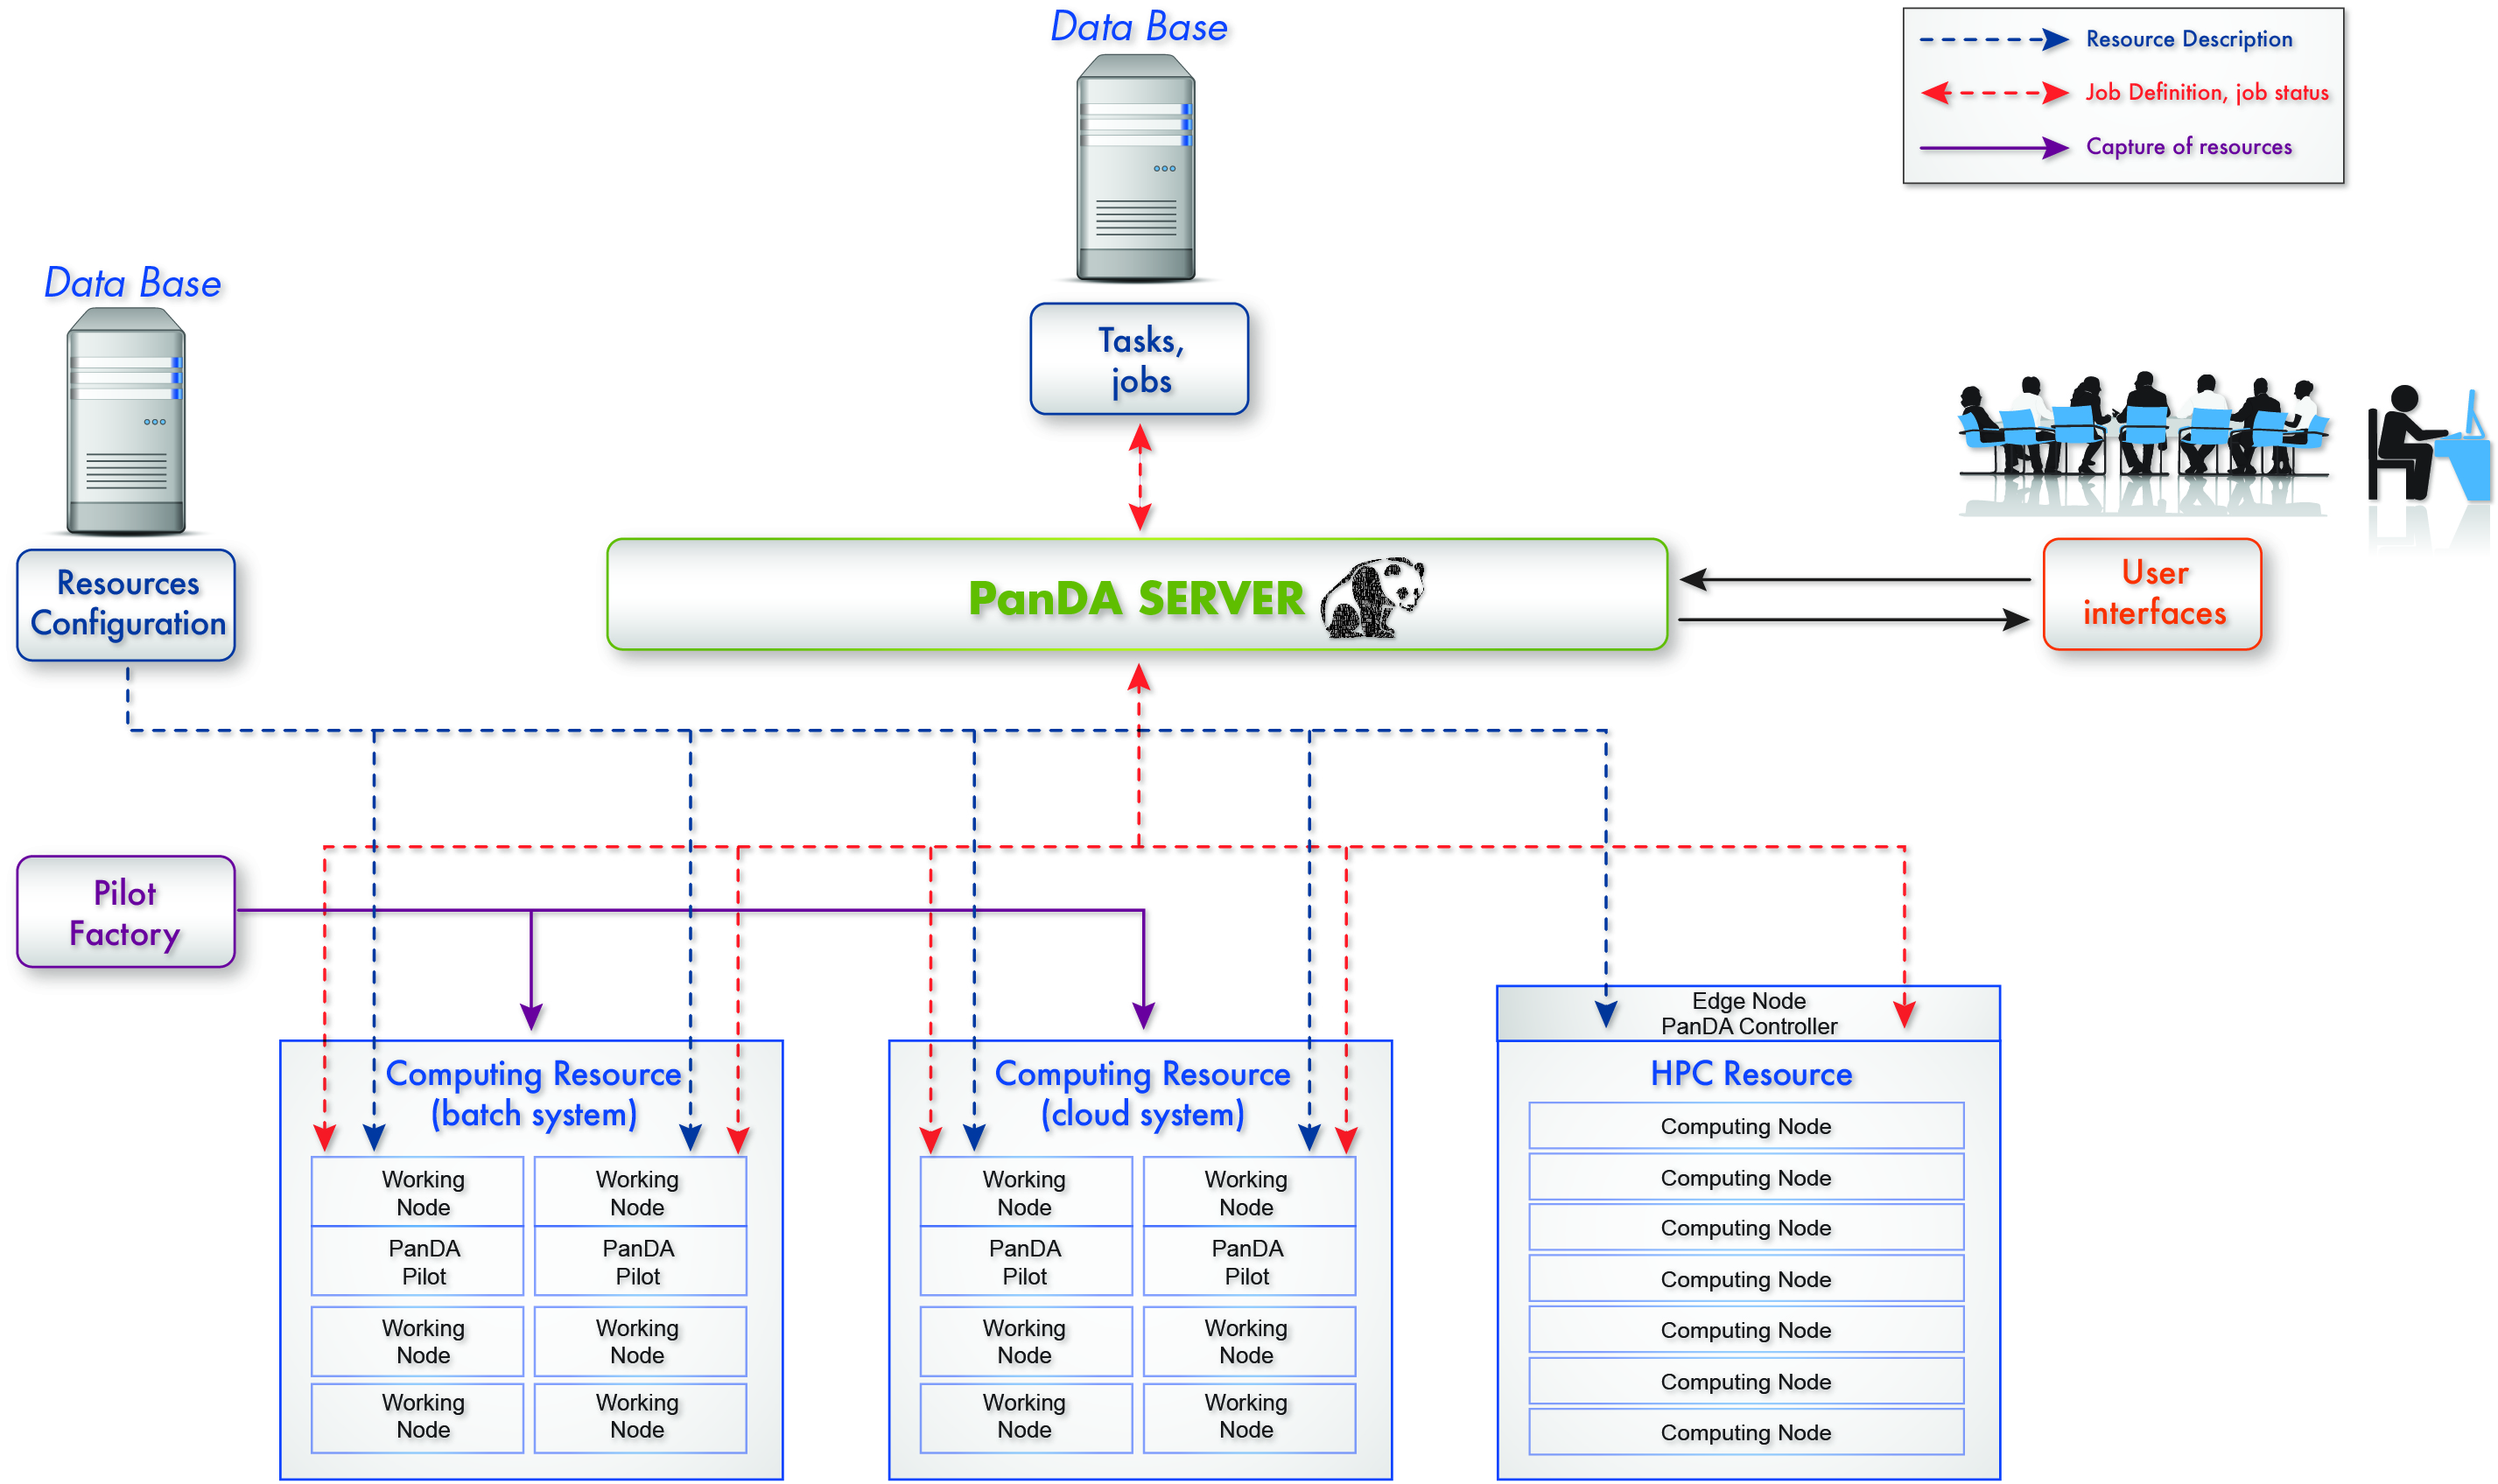
\includegraphics[width=\columnwidth]{figures/PandaArch.jpg}
\caption{Schematic view of the PanDA system\label{fig:architecture}}
\end{center}
\end{figure}
\subsection{PanDA Server}
The PanDA server is the main component of the system, It provides  a task queue managing all job information centrally. The PanDA  server receives jobs through the client interface into the task queue, upon which a brokerage module  operates to prioritize  and assign work on the basis of job type, priority, input data and its locality, and available CPU resources. The PanDA  server operates as a web service. It runs on Apache web server, interacting with the back-end database running  on separate servers. It uses the Apache worker  model, with many independent   processes  handling client requests  in  parallel. Since all  state is maintained  in  the central database,  the PanDA Server application instance itself is stateless. Currently production version of PanDA utilizes Oracle database backend, but PanDA  can also work with MySQL family of databases.

\subsection{PanDA Pilot}
 PanDA is a pilot based workload  management system. In the PanDA job lifecycle, pilot jobs (Python scripts that organize workload processing on a worker  node) are submitted to sites. When these  pilot jobs start on a  worker node they contact a central  server  to retrieve  a real payload (i.e., an end-user job) and execute it. Using these pilot-based  workflows helps to improve job reliability, optimize resource utilization, allows for opportunistic  resources usage, and mitigates  many of the problems  associated with the inhomogeneities found on the Grid.
The pilots themselves  do not contain all the functionality needed to request a payload  job from the Panda Server. First, the complete  set of pilot code is downloaded via HTTP from a  central Subversion repository.  The repository works with Apache web server configured  with a  memory-based   web proxy (Squid). The purpose  of the cache  is to reduce  the request load on the back-end Subversion  server. That allows for a  very good performance since only occasional  queries trigger a  full  lookup on the back-end  Subversion  system, and most external  queries are pulled from memory on the front-end web server. The benefits of this system include a high-performance code download service combined with code updates still being immediately  available  as soon as they are committed to source code control.

\subsection{PanDA Factory}
As a pilot-based  system, PanDA  requires some way to get the initial PanDA pilot onto worker nodes at sites. This is done with the help of a component  called AutoPyFactory (APF). APF runs in a single daemonized process, launching  a separate thread for each internal  workflow. Each one of these internal workflows typically serves  a single job queue  as defined  in WMS, and delivers pilots to a single batch queue, either local or remote. The behavior of these APF workflows is determined by the combination of a set  of plugins, invoked in a  fixed order, in a loop, each one in charge of the performance of a well defined action.

\subsection{PanDA Monitoring}
The PanDA Monitor is a web-based dashboard-style  graphical application. It runs on Apache and interacts with the back-end database for persistence. The Monitor is the primary way that users and site administrators get a  view into the status of current and past jobs, data movement,  pilot factory. The Monitor allows users  access  to all job log files on job by job basis thus greatly simplifying code debugging and failure analysis in distributed computing environment.

\section{Evolution of PanDA WMS}
While PanDa  currently uses  more than 100,000  cores at well over 100 Grid sites with a  peak performance  of 0.3 petaFLOPS,  next LHC data taking run will  require more resources  than Grid computing can possibly provide. The Worldwide LHC Computing Grid (WLCG) infrastructure will be sufficient for the planned analysis and data processing, but it will be insufficient  for Monte Carlo (MC) production and any extra activities. Additional computing and storage  resources are therefore required.  To alleviate  these challenges, ATLAS is engaged  in an ambitious  program to expand  the current computing model to include  additional  resources such as the opportunistic   use of supercomputers   as well as commercial and academic clouds. In turn this activity drives evolution of the PanDA WMS.

\subsection{Use of Supercomputers with PanDA}
The idea is to extend the ATLAS Computing Model beyond the Grid into the domains of supercomputers. Modern High Performance Computing  (HPC) involves  a very large number of worker nodes  connected  through a  high-speed   network. The worker nodes can have  multicore CPUs that can be augmented with massively parallel Graphics Processing Units (GPUs) or other types of coprocessors. On an HPC machine, a  typical job is highly parallel and connected,  where each core calculates  a small part of the problem and coordinates the activity via message passing interface (MPI). While this is different from the HEP computing paradigm, where jobs are independent, it still shares common  features  such as the use of parallelization. It is not a requirement  that HPC machines are able to run any possible task, nor is it relevant how many kinds of job types that can be run. What matters is the total number of cycles that can be offloaded from the Grid. Standard  ATLAS  workflow  can not be easily ported to supercomputers   due  to   several   complications such  as specialized worker  node  setups, no  outbound network connections,  limited memory per node, custom operating systems,  etc. A reorganization  of the standard  workflow is therefore needed.
The most suitable task for HPCs in HEP is event generation. Event generators are mostly computational,  stand-alone code, with few input requirements.  There is no need  to stage-in much data. The event generation  in ATLAS corresponds  to
10-15\% of all jobs on the Grid. A more difficult workload to adapt  for HPCs is detector  simulation. Simulation tasks tend to be tied to the framework of a particular simulation and often require  database access for geometry and relevant run conditions.  However,  there is a  lot to be gained  since simulation  tasks correspond to 2/3 of the Grid capacity.
\subsection{Interfacing PanDA with Titan}
The Titan supercomputer, current number two (number one from November 2012 until June 2013) on the Top 500 list is located at the Oak Ridge Leadership Computing  Facility (OLCF) in Oak Ridge National Laboratory, US. Titan, was the first large-scale system to use  a hybrid architecture that utilizes worker nodes with both AMD 16-core Opteron 6274 CPUs and NVIDIA Tesla K20 GPU accelerators.
Integration with Titan is the current focus for PanDA developers. The project aims to integrate Titan with the PanDA system using an updated PanDA Pilot that runs on the front-end node and submits ATLAS payloads to the worker nodes using the local batch system (PBS) via the SAGA (Simple API for Grid Applications) interface \cite{SAGA}. This solves several complications of  running on HPC worker nodes,  including the lack of connectivity to outside world. The pilot can communicate with the PanDA server from the front-end machine. The interactive front-end  machines and the worker nodes  use  a shared  file system  which makes  it  easy  for the pilot to stage-in  any input files that are required by the payload and stage-out the produced output files after the payload has finished at the end of the job. ATLAS Tier 1 computing  center at Brookhaven National Lab is currently  used for data stage out from Titan but in principle  that can be any Grid site.
1) HPC Backfill: HPC facilities are geared towards  large scale jobs by design. Time allocation on an HPC is competitive and large projects are often preferred. About 10% of capacity on a  typical HPC machine  is unused  due to mismatches between job sizes and available  resources. The worker nodes
\begin{figure}
\begin{center}
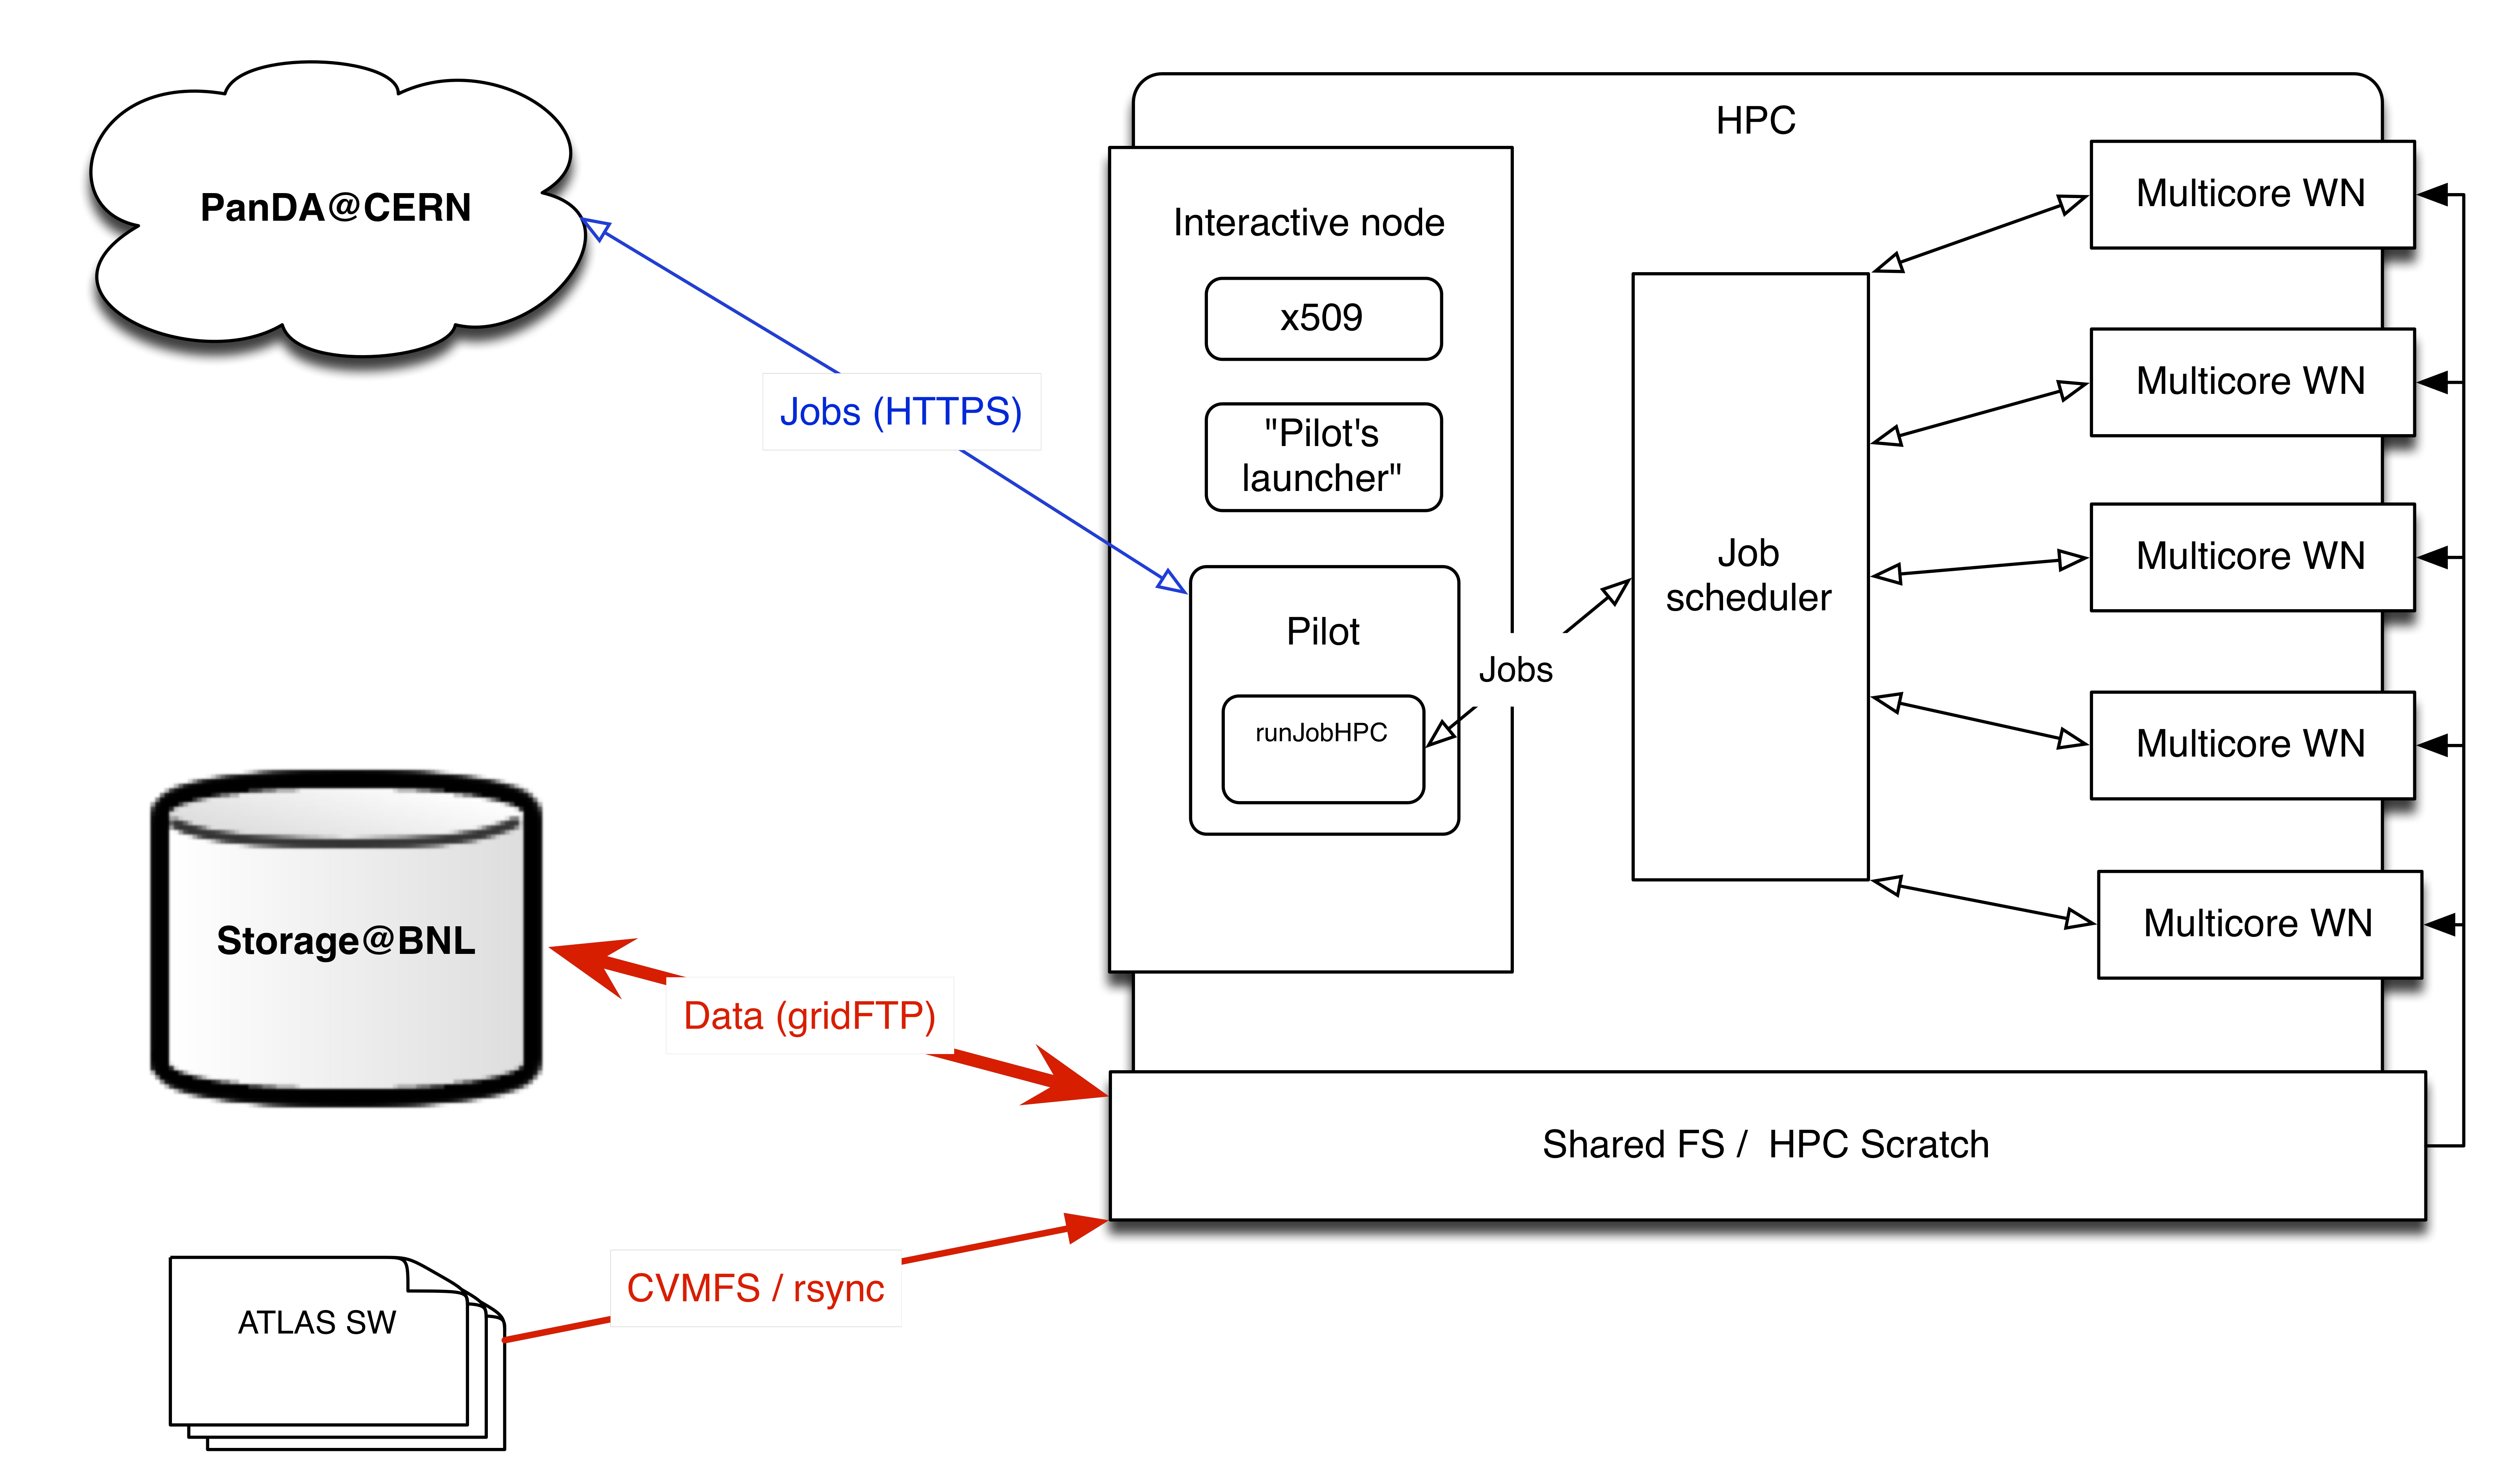
\includegraphics[width=\columnwidth]{figures/PandaInterfaceWithHPC.png}
\caption{Schematic view of the PanDA system\label{fig:interface}}
\end{center}
\end{figure}


--------------------------------------------------------------------
\begin{enumerate}
  \item PanDA WMS
  \begin{enumerate}
    \item State Diagrams
    \item Control Flow Diagrams
    \item Software Module and Architecture diagrams.
  \end{enumerate}
  \item PANDA Pilot
\end{enumerate}

% ----------------------------------------------------------------------------
% V
% ----------------------------------------------------------------------------
\section{Deploying PanDA on a Leadership-scale system}
\label{sec:panda_deployment}

\begin{enumerate}
  \item Challenges
  \item Opportunities
  \item Highlight distinction of PanDA on wide-area distributed systems vs on TITAN
  \item Take-aways, lessons learned
\end{enumerate}

% ----------------------------------------------------------------------------
% VI
% ----------------------------------------------------------------------------
\section{Performance Characterization}
\label{sec:panda_performance}

\begin{enumerate}
  \item Internal PanDA performance
  \item External PanDA performance (workload specific on underlying system/platform)
\end{enumerate}

% ----------------------------------------------------------------------------
% VII
% ----------------------------------------------------------------------------
\section{Putting it all together: Experience of PanDA on TITAN} % (fold)
\label{sec:panda_titan}

\begin{enumerate}
  \item Metadata performance issue, and how it’s resolved
  \item File I/O performance and impact
  \item ?
\end{enumerate}

% ----------------------------------------------------------------------------
% VIII
% ----------------------------------------------------------------------------
\section{PANDA: Future/RoadMap}
\label{sec:panda_roadmap}

 \section{Conclusion}\label{sec:conclusion}
The PanDA  system was developed to meet the scale and complexity of LHC distributed computing for the ATLAS experiment.  In the process,  the old batch job paradigm  of computing in HEP was  discarded  in favor of a  far more flexible and scalable  model. The success  of PanDA  at the LHC is leading to widespread adoption and testing by other experiments. PanDA  is the first exascale  workload management system in HEP, already operating at a million computing jobs per day, and processing over an exabyte of data in 2013. Next LHC run will pose massive computing  challenges. With a  doubling of the beam  energy  and luminosity as  well as an increased  need for  simulates  data, the data volume is expected to increase with a factor 5-6 or more. Storing and processing  this amount of data is a  challenge   that cannot be resolved with the currently existing  computing  resources in ATLAS. To resolve this challenge, ATLAS is turning to commercial  as well as academic Cloud services and HPCs via the PanDA system. Also the work underway is enabling the use of PanDA by new scientific collaborations and communities as a means  of leveraging  extreme scale computing  resources with a low barrier of entry. The technology base provided by the PanDA system will enhance the usage of a variety  of high-performance computing resources available to basic research.



\section*{Acknowledgements}
\label{sec:ack}

The authors would like to thank... More thanks here...

This research used resources of the Oak Ridge Leadership Computing Facility,
located in the National Center for Computational Sciences at the Oak Ridge
National Laboratory, which is supported by the Office of Science of the
Department of Energy under Contract DE-AC05-00OR22725.

What other boilerplate text is needed?




%\section*{Acknowledgment}

%The authors would like to thank... More thanks here...

% trigger a \newpage just before the given reference
% number - used to balance the columns on the last page
% adjust value as needed - may need to be readjusted if
% the document is modified later
%\IEEEtriggeratref{8}
% The "triggered" command can be changed if desired:
%\IEEEtriggercmd{\enlargethispage{-5in}}

% references section

% can use a bibliography generated by BibTeX as a .bbl file
% BibTeX documentation can be easily obtained at:
% http://www.ctan.org/tex-archive/biblio/bibtex/contrib/doc/
% The IEEEtran BibTeX style support page is at:
% http://www.michaelshell.org/tex/ieeetran/bibtex/
%\bibliographystyle{IEEEtran}
% argument is your BibTeX string definitions and bibliography database(s)
%\bibliography{IEEEabrv,../bib/paper}
%
% <OR> manually copy in the resultant .bbl file
% set second argument of \begin to the number of references
% (used to reserve space for the reference number labels box)

\bibliographystyle{plain}
\bibliography{bibliography}

% that's all folks
\end{document}


